\documentclass[border=2pt]{standalone}
\usepackage{tikz}
\usetikzlibrary{angles,quotes}
\usepackage{amsmath}
\begin{document}


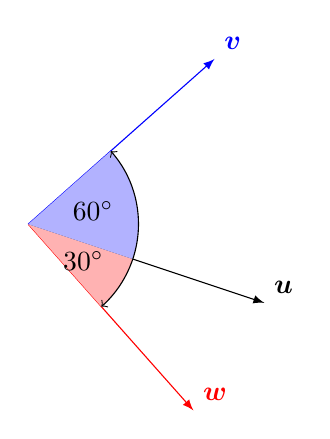
\begin{tikzpicture}[angle radius=1.4cm]
	% \draw[-latex] (0,0)--(3,1);
	\draw[-latex] (0,0) coordinate (A) -- (3,-1) coordinate (B) node[anchor=south west]{$\boldsymbol{u}$};
	\draw[-latex, red] (0,0) to ({atan(-1/3)-30}:{sqrt(10)}) coordinate (C) node[anchor=south west]{$\boldsymbol{w}$};
	\draw[-latex, blue] (0,0) to ({atan(-1/3)+60}:{sqrt(10)}) coordinate (D) node[anchor=south west]{$\boldsymbol{v}$};
	\draw pic ["$30^\circ$", draw, <-, fill=red!30] {angle = C--A--B};
	\draw pic ["$60^\circ$", draw, ->, fill=blue!30] {angle = B--A--D};
\end{tikzpicture}

\end{document}
